\documentclass[a4paper]{article}
\usepackage{natbib}
\usepackage{hyperref}
\hypersetup{
    colorlinks,
    citecolor=black,
    filecolor=black,
    linkcolor=black,
    urlcolor=black
}
\usepackage{graphicx}
\usepackage[english]{babel}


\begin{document}
	\begin{titlepage}
\begin{center}
\textsc{\LARGE Contextproject Programming Life}\\
\vspace{5pt}
\textsc{\LARGE Group 2 - GEVATT}\\
\vspace{5pt}
\textsc{\LARGE Final Report}\\
\vspace{5pt}
\textsc{\large TU Delft}

\begin{table}[ht]
\centering
\begin{tabular}{ccc}

\includegraphics[scale=0.2]{ruben.png}   &
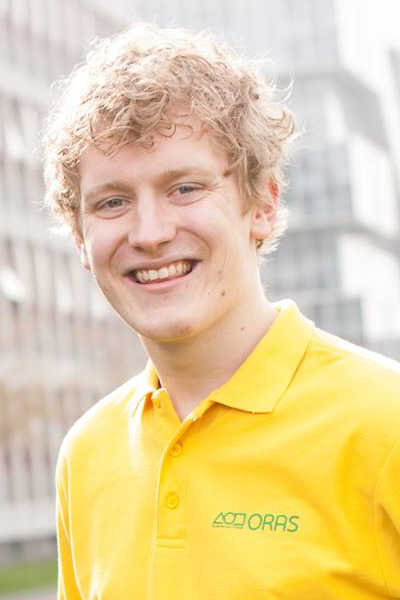
\includegraphics[scale=0.2]{mathijs.png} &

\includegraphics[scale=0.2]{jasper.png}  \\
Ruben Bes	& Mathijs Hoogland	& Jasper Denkers\\
rbes 		& mhhoogland 		& jdenkers\\
4227492 	& 4237676 			& 4212584\\
\end{tabular}
\end{table}

\begin{table}[ht]
\centering
\begin{tabular}{cc}
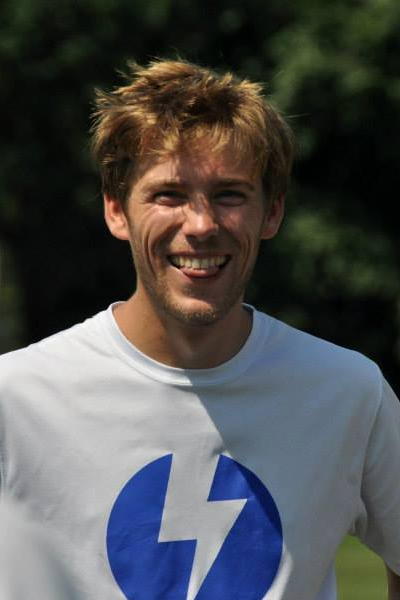
\includegraphics[scale=0.2]{robbert.png} &

\includegraphics[scale=0.2]{willem.png}  \\
Robbert van Staveren	& Willem Jan Glerum\\
rhvanstaveren 			& wglerum\\
1527118					& 4141040\\
\end{tabular}
\end{table}

\vfill
{\large \today}
\end{center}

\end{titlepage}
	
	\begin{abstract}
		\textless Insert Abstract Here\textgreater
	\end{abstract}
	\clearpage
	
	\tableofcontents
	\clearpage
	
	\section{Introduction}
		This document provides information on the system that will be built during the context project programming life. We have also set up a couple of goals which will be followed as much as possible. The architecture of the product will be discussed in the form of high level components. These may be split up into subcomponents and/or subsystems.
		\subsection{Design goals}
		Our product will focus on:
		\begin{itemize}
			\item Availability
				\subitem We plan to have a working system at all times, with more functionality being added each week. Using this approach, our customer can try the product after each iteration, resulting in feasible feedback which we can use to quickly alter course.
			\item Manageability
				\subitem Doctors will not have to manage anything, as they have no direct access to the databases or any data. They will only be provided visualizations to interact with.
			\item Ease of use
				\subitem Since our application runs on a server and a doctor can access our data with a web page, no extra programs are required. The user will log on with his credentials and can select a vcf-file to upload to our server as well as provide some data on the trio.
			\item Performance
				\subitem As vcf-files are quite large, the data will be sent to the server while the doctor can still access the website. The data can be analysed quickly by the server and the results will be returned and locally visualized.
			\item Scalability
				\subitem Our application will be scalable in a sense that multiple users can upload files. However the databases containing information about the genetic variations (string, dbSNP and CADD) will continue to grow and thus the computational power required to gather the information needed will also grow. This however is not the problem of our server, but of the host of the server.
			\item Reliability
				\subitem The application should be very reliable, as servers are generally always on. The user only needs to connect to the web page.
			\item Secureness
				\subitem Doctors are required to log onto our system via the web page, thus unauthorized access is prevented. The data sent over will only be saved for a short time, long enough for it to be analyzed. After this it is deleted and the results are submitted.
		\end{itemize}
		\subsection{Programming languages and programs}
		
	\section{Software architecture views}
		This section discusses the system's architecture. It is composed of subsystems which depend on one another, this will be explained in the first subsection. The second subsection focuses on the relation between the hard- and software. Finally, the third subsection discusses the management of data used by the product.
		\subsection{Subsystem decomposition}
			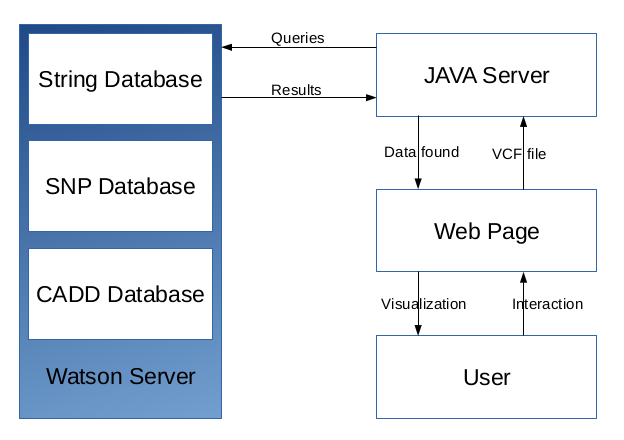
\includegraphics[scale=0.5]{schema1.png}
			\begin{itemize}
				\item Watson server
					\subitem The Watson server hosts the databases string, dbSNP and CADD and processes queries given by the JAVA server and returns the results.
				\item JAVA server
					\subitem The JAVA server makes queries and sends these to Watson. It makes these based on the VCF-file given by the web page. It processes these and determines which data is to be retrieved. The data retrieved is then sent to the web page.
				\item Web page
					\subitem The web page receives the vcf-file from the user and passes it on to the JAVA server. When it receives data back from the server it visualizes this for the user.
				\item The user 
					\subitem The user can interact with the web page and pick a VCF-file to send. The web page outputs a visualization and the user can draw conclusions from this.
			\end{itemize}
		\subsection{Hardware/software mapping}
			This system will only be used by one type of person, namely a doctor. This means that only one interface will have to be developed and used. A user needs to log on to a web page, after which he or she will be shown a page where VCF-files can be uploaded and analyzed. The web page can be accessed from devices connected to the internet but is targeted at desktops.
		\subsection{Persistent data management}
			The only data our application handles are VCF-files sent by users. We currently have no plans to fill a database with these files for each user. We might give the user the option to export the data of the visualization so that he or she can view this later. We try to keep the data in the JAVA server as low as possible, to support more users.
		\subsection{Concurrency }
			At the moment we have no indication how computationally intense our calculations are, thus we cannot say for sure whether or not we will use multiple threads. Until we know more, our program will run on a single thread.
			
	\section{Glossary}
		\begin{itemize}
			\item SNP
				\subitem Single Nucleotide Polymorphism, a single change in DNA compared to the reference. genome
			\item git
			\item vcf
			\item triodata
		\end{itemize}
\end{document}